%% Template article for Elsevier's document class `elsarticle'
%% with numbered style bibliographic references
\documentclass[preprint,12pt]{elsarticle}

% remove preprint footnote
\makeatletter
\def\ps@pprintTitle{%
 \let\@oddhead\@empty
 \let\@evenhead\@empty
 \def\@oddfoot{\centerline{\thepage}}%
 \let\@evenfoot\@oddfoot}
\makeatother


\usepackage{setspace}
\doublespacing

\usepackage{hyperref} % auto detect ref type
\usepackage{natbib}
\setcitestyle{authoryear}

%% Use the option review to obtain double line spacing
%% \documentclass[preprint,review,12pt]{elsarticle}

%% Use the options 1p,twocolumn; 3p; 3p,twocolumn; 5p; or 5p,twocolumn
%% for a journal layout:
%% \documentclass[final,1p,times]{elsarticle}
%% \documentclass[final,1p,times,twocolumn]{elsarticle}
%% \documentclass[final,3p,times]{elsarticle}
%% \documentclass[final,3p,times,twocolumn]{elsarticle}
%% \documentclass[final,5p,times]{elsarticle}
%% \documentclass[final,5p,times,twocolumn]{elsarticle}

\usepackage{graphicx}
\usepackage{amssymb}
\usepackage{amsmath}
\usepackage{caption}
\usepackage{textcomp}    % for Hawaii characters

\biboptions{comma,round}

% shortcuts
\newcommand{\bbeta}{\boldsymbol{\beta}}
\newcommand{\blambda}{\boldsymbol{\lambda}}
\newcommand{\T}{\intercal}
\newcommand{\bS}{\mathbf{S}}
\newcommand{\bQ}{\mathbf{Q}}
\newcommand{\bSigma}{\boldsymbol{\Sigma}}
\newcommand{\bm}{\boldsymbol}  % bold maths symbols
\newcommand{\tl}{\tilde{\lambda}}   % thinned little lambda
\newcommand{\tL}{\tilde{\Lambda}}  % thinned big lambda

% RJC 09/08/2019 Added shortcuts for Hawaiian words
\newcommand{\akepa}{\textquotesingle\={a}kepa}  % adds Hawaiian diacritical marks
\newcommand{\Akepa}{\textquotesingle\={A}kepa}  % adds Hawaiian diacritical marks
\newcommand{\hawaii}{Hawai\textquotesingle i}   % adds Hawaiian diacritical marks
\DeclareMathOperator*{\argmax}{arg\,max}  % * means _ puts thing beneath operator

\begin{document}
\begin{frontmatter}
\title{Point transect distance sampling in inlabru}

%% use the tnoteref command within \title for footnotes;
%% use the tnotetext command for the associated footnote;
%% use the fnref command within \author or \address for footnotes;
%% use the fntext command for the associated footnote;
%% use the corref command within \author for corresponding author footnotes;
%% use the cortext command for the associated footnote;
%% use the ead command for the email address,
%% and the form \ead[url] for the home page:
%%
%% \title{Title\tnoteref{label1}}
%% \tnotetext[label1]{}
%% \author{Name\corref{cor1}\fnref{label2}}
%% \ead{email address}
%% \ead[url]{home page}
%% \fntext[label2]{}
%% \cortext[cor1]{}
%% \address{Address\fnref{label3}}
%% \fntext[label3]{}


%% use optional labels to link authors explicitly to addresses:
%% \author[label1,label2]{<author name>}
%% \address[label1]{<address>}
%% \address[label,2]{<address>}

% RJC 09/08/2019 Added co-authors and affiliations. Note that I used \affil[]{} instead of \address[]{}
\author[1,*]{Andrew E Seaton}
\author[1,2]{Richard J Camp}
\author[3]{Finn Lindgren}
\author[1]{Janine B Illian}
\author[1]{David L Borchers}
\author[1]{David L Miller}      % Ask about co-authoring the manuscript
\author[1]{Len Thomas}          % Ask about co-authoring the manuscript
\author[1]{Stephen T Buckland}  % Ask about co-authoring the manuscript
\author[4]{Steve J Kendall}     % It is Steve's data we are using and I have already mentioned this manuscript to him.

%\address{Centre for Research into Ecological \& Environmental Modelling and School of Mathematics \& Statistics, University of St Andrews, St Andrews, Fife, Scotland}
\address[1]{Centre for Research into Ecological \& Environmental Modelling and School of Mathematics \& Statistics, University of St Andrews, St Andrews, Fife, Scotland}
\address[2]{U. S. Geological Survey, Pacific Island Ecosystems Research Center, P.O. Box 44, \hawaii{} National Park, HI 96718, U.S.A.}
\address[3]{School of Mathematics, University of Edinburgh, Edinburgh, Scotland}
\address[4]{U. S. Fish and Wildlife, Big Island National Wildlife Refuge Complex, 60 Nowelo St., Suite 100, Hilo, HI  96720, U.S.A.}
\address[*]{Correspondence: Andrew E Seaton, Email: aes22@st-andrews.ac.uk}

\begin{abstract}
Point transect distance sampling in \texttt{inlabru}
\end{abstract}

%\begin{keyword}
%Distance sampling \sep Stochastic partial differential equations \sep Integrated nested Laplace approximation \sep Generalized additive model
%\end{keyword}
\end{frontmatter}

\section*{Introduction}

The estimation of the size of wild populations of animals is a critical objective within ecology and conservation \citep{schwarz_estimating_1999}.  Distance sampling methods aim to achieve this by using a spatially explicit sampling design and estimating the detectability of animals as a function of distance from observer \citep{buckland_advanced_2008, buckland_distance_2015}.  Standard distance sampling approaches use a hybrid of design- and model-based inference to estimate population size.  Probability of detection is modelled as a function of distance from observer and a randomized sampling design allows the construction of Horvitz-Thompson-like estimators of animal density \citep{horvitz_generalization_1952,  buckland_advanced_2008}.

Over time interest grew in fully model-based approaches which allow the use of non-randomized survey designs by considering a spatial model for animal density.  This allows observations to be associated with spatially indexed covariates and abundance can, in principle, be estimated for any subregion within the study area \citep{johnson_model-based_2010, miller_spatial_2013, buckland_model-based_2016}.  
Model-based distance sampling has typically been implemented in a two-stage modelling process.  In the first stage, detectability is estimated within each sampling unit.  In the second stage, detections within sampling units are binned into counts and used as the response variable in a generalized additive model framework where the detectability estimates from the first stage are used as an offset.  Due to often sparse nature of wildlife survey data this may require consideration of over or under-dispersion and zero-inflated distributions.  Negative-binomial and Tweedie distributions are common choices to model the distribution of counts \citep{wood_gam_2017}.

A key concern with the two-stage approach is the propagation of the uncertainty in the detectability estimates to the second-stage spatial model.  Early attempts to address this focused on bootstrapping \citep{lahiri_resampling_2003}, but more recent work with the bootstrapping approach has pointed to potentially irresolvable difficulties that require resampling blocks at multiple spatial scales. Instead \cite{bravington_reliable_2018-1} proposed propagating error based on a second-order Taylor approximation of detectability around the maximum-likelihood estimate from the first stage.

\citet{yuan_point_2017} presented a one-stage approach for analysing line-transect distance sampling within a Bayesian framework that simulateously estimates the detectability 
and spatial distribution of animals.  Key to their approach is the use of a sparse Gaussian Markov random field (GMRF) approximation to a continously-indexed Gaussian random field (GRF) and a log-Gaussian Cox point process model that avoids the need to bin data into counts and naturally sidesteps issues of zero-inflation and dispersion.  The observation process is formulated as a thinning of the log-Gaussian Cox process.  Both the log-intensity of points and the detection function were modelled using a stochastic partial differential equation (SPDE) approach \citep{lindgren_explicit_2011}.  The model was specified as a latent Gaussian model and fitted using integrated nested Laplace approximations using the \texttt{R-INLA} package \citep{rue_approximate_2009}.  

Here we present a similar approach to \citet{yuan_point_2017} but instead focus on the case of point transect data and replace the SPDE specification of the detection function with a parametric family of detection functions which are familiar to users of standard distance sampling methods.  Point transects require special treatment to account for the fact that the area surveyed increases with increasing distance from the observer.  Our case study is, to the best of our knowledge, the first analysis of point transect distance sampling data formulated as a thinned point process.  However, the point process viewpoint is not new and has been applied numerous times to line transect data \citep{buckland_model-based_2016, johnson_model-based_2010, hedley_spatial_2004, stoyan_remark_1982, hogmander_random_1991}.  We also present the first use of a sparse GMRF spatial random effect with point transect distance sampling data.  The sparsity of the GMRF is useful for computational efficiency and the finite element mesh motivated by the SPDE allows efficient handling of complex spatial domains such as coastlines \citep{simpson_going_2016}.   

To demonstrate the benefits of this one-stage approach we highlight potential issues regarding model evaluation and communication of results that are common in many formulations of species distribution modelling.  We discuss potentially misleading summary maps of the posterior intensity process and propose an alternative based on excursion sets \citep{bolin_excursion_2015, bolin_calculating_2018}.  A key theme in our case-study is to highlight the importance of considering \textit{realizations} of random quantities rather than rely too much as summaries such as expectations and quantiles.  The one-stage approach is invaluable since model summaries are based on monte-carlo sampling from the joint posterior of all model parameters.  Since the spatial process and observation process are estimated jointly this means figures and summaries produced naturally average over the estimated uncertainty in the observation processes.  This is an advantage over the two-stage approach even if uncertainty has been effectively propagated in some way.  

The article proceeds as follows.  First we present the perspective of point transect distance sampling as a thinned poisson process, describing in detail how this can be formulated as a latent Gaussian model with a latent GMRF random effect.  We also show how the point process viewpoint can still be used in the case of incomplete location information where only the distance from the observer is recorded, not the exact location of the animal.  Secondly we describe how to specify the joint model using an iterative approach to fitting models with components that are non-linear in their parameters.  Thirdly, we introduce our case-study using a point transect distance sampling survey of the Hawaiian \akepa{}, an endangered bird of the honeycreeper tribe.  We show how the above methods can be specified and fit using the software package \texttt{inlabru} \citep{bachl_inlabru_2019}, an extension of the \texttt{R-INLA} package. We focus our model evaluation on the effective understanding and communication of uncertainty in the posterior intensity and abundance estimates, which are typically of greatest interest to stakeholders.


\section*{Distance Sampling as a Thinned Point Process}

We assume the location of animals are a point pattern that follows a log-Gaussian Cox process with intensity process $\lambda(s)$.  The log-Gaussian Cox process is a flexible approach that can include spatially structured random effects on the intensity process to account for unexplained heterogeneity not captured by fixed effect covariates.

\sloppy For the case with imperfect detection of points we specify a thinning probability function $g(s) = \mathbb{P}(\text{a point at $s$ is detected})$. A key property of the log-Gaussian Cox process is that a realisation of a point process with intensity process $\lambda(s)$ that is thinned by thinning probability function $g(s)$ also follows a log-Gaussian Cox process with intensity given by $\tl(s) = \lambda(s)g(s)$.

Standard distance sampling approaches specify $g(s)$ as a function that decays with increasing distance from the observer.  For example, if $r(s)$ denotes the distance of a point at $s$ from the observer, the half-normal thinning probability function is $g(s | \sigma) = \exp(-r(s)^2 / 2\sigma^2)$ where $\sigma$ is a variance parameter to be estimated using the observed distances.  The parameter $\sigma$ can only be estimated if an assumption is made about the intensity of the animal locations.  Without such an assumption detectability and intensity are confounded.  The standard assumption of distance sampling is that the intensity is constant with respect to changes in $r(s)$.  Thus any observed differences from uniformity can be attributed to detectability, and not variation in the intensity.

A point transect distance sampling survey consists of a set of $K$ sampled regions.  The $k$-th sampled region we denote $\Omega_k \subset \mathbb{R}^2$ and the total surveyed region $\Omega = \cup_{k=1}^K \Omega_k$.  For simplicity we assume that all sampled regions are discs with radius $W$ and $\Omega_j \cap \Omega_k = \emptyset$ for all $j \neq k$.  The thinning probability function $g(s)$ is then defined relative to the positions of the surveyed regions.  We denote the probability of observing a point $s \in \Omega_k$ as $g_k(s)$.  The probability of observing a point outside the surveyed region is zero.  [RJC - I switched the order of the two previous sentences. That way we start with the relevant probability, followed by defining the probability elsewhere is zero]  Since the surveyed regions are non-overlapping each location $s$ is associated with a single thinning probability function $g_k$.  For example, for an observer at location $s_k \in \Omega_k$, the half-normal thinning probability function is $g_k(s) = \exp(-\lVert s - s_k \rVert_2^2 / 2\sigma^2)$. The assumption of non-overlapping survey regions can be relaxed by including extra information such as the time of each observation.  For simplicity we do not consider this here.  The thinning probability function for any $s \in \Omega$ is then given by $g(s) = g_{k(s)}(s)$ where $k(s) = k$ for $s \in \Omega_k$.

The likelihood of observed points at locations $\bm{Y} = (s_1, \ldots, s_n)^\intercal$ is then
\begin{equation}
\label{lgcp-likelihood}
\pi(\bm{Y} | \theta, \phi) = \exp\left(-\int\displaylimits_{s \in \Omega} \lambda(s) g(s) \mathrm{d}s \right)\prod_{i=1}^n \lambda(s_i)g(s_i)
\end{equation}

The integral component of the likelihood does not usually have analytical solutions.  Replacing the integral with a weighted sum allows the log-likelihood to be rewritten as a weighted Poisson log-likelihood.

To evaluate the integral we introduce polar coordinates notation $s_k(r, \theta) = s_k + r\left[\cos\theta, \sin\theta \right]^T$ to represent locations in each sampling unit $\Omega_k$.   In general the thinning function depends only on $r$ and not on $\theta$.  We assume this is the case in the following and use the shorthand $g_k(r) = g(s_k(r, \theta))$. It follows that the integral can be rewritten as a sum of weighted one-dimensional integrals $\sum_{k=1}^K 2\pi \lambda(s_k) \int_0^W r g_k(r)\mathrm{d}r$ using the assumption that $\lambda(s)$ is constant within each sampling unit.  For each sampling unit we approximate the one-dimensional integral using a midpoint integration method with $M$ integration locations $r_{k1}, \ldots, r_{kM}$ and associated weights $\alpha_{k1}, \ldots, \alpha_{kM}$.  This gives
\begin{equation*}
	\int\displaylimits_{s \in \Omega} \lambda(s)g(s)\mathrm{d}s \approx \sum_{k=1}^K \sum_{j=1}^M \tilde{\alpha}_{kj} \tl(s_{kj})
\end{equation*}
where $\tilde{\alpha}_{kj} = 2\pi \alpha_{kj}r_{kj}$ and $\tl(s_{kj}) = \lambda(s_k) g_k(r_{kj})$.

To simplify notation below we let $\tilde{\alpha}_{k} = (\alpha_{k1}, \ldots, \alpha_{kM})^\intercal$ and $\tilde{\alpha} = (\alpha_1^\intercal, \ldots, \alpha_K^\intercal)^\intercal$.  Similarly let $\tl_k = (\tl(s_{k1}), \ldots, \tl(s_{kM}))^\intercal$, $\tl_{int} = (\tl_1^\intercal, \ldots, \tl_K^\intercal)^\intercal$ and denote the intensity evaluated at the observed locations as $\tl_{obs} = (\tl(s_1), \ldots, \tl(s_n))^\intercal$

Then the approximate log-likelihood is

\begin{equation}
\label{approx-log-likelihood}
	\log \pi(\bm{Y}) \approx - \tilde{\alpha}^\intercal \tl_{int} + 1^\intercal\log\tl_{obs}
\end{equation}

This approximation can be written as a modified Poisson likelihood.  To see this let $\exp \eta = (\tl_{int}^\intercal, \tl_{obs}^\intercal)^\intercal$,
$\alpha = (\tilde{\alpha}^\intercal, 0_{n \times 1}^\intercal)^\intercal$ and construct a vector of pseudo-observations $y = (0_{KM\times 1}^\intercal, 1_{n \times 1}^\intercal)^\intercal$.  Then the approximate likelihood becomes
\begin{equation}
\pi(\bm{Y}) \approx \prod_{i=1}^{KM + n} \eta_i^{y_i}\exp(-\alpha_i\eta_i)
\end{equation}

This is similar to a Poisson likelihood with an offset term equal to $\log\alpha$ and can be specified using the Poisson likelihood implementation available in \texttt{R-INLA}.


\section*{Intensities for incomplete data}

In the above we assume the data are complete records of animal location.  However, in many distance sampling surveys only the location of the observer and the distance to the observer are recorded.  Data of this type can be analysed within a point process framework by deriving the appropriate intensity function for the incomplete data.

Using the polar coordinates notation given above, for true animal location $s_k(r, \theta) \in \Omega_k$ we consider the case where we observe $r$ but not $\theta$.  It follows that the intensity for points at a distance $r$ observed within sampling unit $\Omega_k$ is
\begin{align}
\tl_k(r) &= \oint\displaylimits_{c_k(r)} \lambda(s)g_k(s)\mathrm{d}s \nonumber \\
&= 2\pi\lambda(s_k)rg_k(r)
\end{align}
 where $c_k(r)$ is a circle of radius $r$ centred at $s_k$ and the second line follows from changing to polar coordinates and the assumption of constant intensity within $\Omega_k$.  This intensity differs from the full data case by including the $2\pi$  term to account for the fact that we do not observe $\theta$ and the additional $r$ term to account for the increasing area surveyed at larger distances.

\section*{Modelling $\lambda(s)$ using the stochastic partial differential equation approach}

To model the intensity of animal locations we use a combination of fixed effects of spatial covariates and a spatially structured random effect.  This allows us to associate distance sampling data with environmental and ecological conditions that may be relevant to understanding the ecology of the species of interest.  For cases where we have insufficient covariates to fully explain the location of animals the spatially structured random effect accounts for additional heterogeneity in the intensity and is required to assume conditional independence between points, given the intensity.

The log-intensity of animal locations is given by
\begin{equation*}
\log \lambda(s) = \beta_0 + \sum_v \beta_v z_v(s) + \xi(s)
\end{equation*}
where $\beta_0$ is an intercept parameter, the $z_v(s)$ are spatially indexed covariates with effect parameters $\beta_v$ and $\xi(s)$ is a zero-mean Gaussian random field with Mat\'ern covariance
\begin{equation}
C(s_1,s_2) = \frac{2^{1-\nu}}{4\pi\kappa^2\tau^2\Gamma(\nu)}(\kappa \|s_1-s_2\|)^{\nu}K_\nu(\kappa \|s_1-s_2\|)
\end{equation}
where \(\nu, \kappa, \tau\) are parameters and \(K_{\nu}\) is the modified Bessel function of the second kind.  All three parameters are not simultaneously identifiable \citep{zhang_inconsistent_2004} and it is conventional to assume a value for $\nu$ which controls the mean-square differentiability of the process.  We set $\nu = 1$ which is the most default value in \texttt{R-INLA}. [[Would like to justify $\nu = 1$ somehow?]]

We use a Gaussian Markov random field approximation of $\xi(s)$ following the approach of \cite{lindgren_explicit_2011} based on specifying $\xi(s)$ via a stochastic partial differential equation.  Given a finite element mesh on the spatial domain with $L$ nodes and associated piece-wise linear basis functions $\phi_1, \ldots, \phi_L$ we represent $\xi$ as $\xi(s) = \sum_l \xi_l \phi_l(s)$.  The parameters $\xi_1, \ldots, \xi_L$ are a Gaussian Markov random field with sparse prior precision matrix $\bm{Q}_{\xi} = \frac{1}{\tau^2}\left(\kappa^4\bm{C} + 2\kappa^2\bm{G_1} + \bm{G_2}\right)$ where $\bm{C}$, $\bm{G_1}$, $\bm{G_2}$ are all sparse matrices the elements of which are defined via an approximate solution to a stochastic partial differential equation. The precision parameter $\tau$ controls the marginal variance of the field and $\kappa$ is an inverse range parameter that controls the rate of decay of the covariance as distance between locations increases.  Further details of this Gaussian Markov random field approximation are given in the supplementary materials.

\section*{Thinned Intensities}

The above specifies a model for all animal locations in the area of interest.  The log-intensity for observed points is $\log\tl(s) = \log\lambda(s) + \log g(s)$.  This presents a problem since $\log g(s)$ is not typically linear in its parameters. However, for any single set of parameter values $g(s)$ can be viewed as acting like an offset. If we could specify $g(s)$ as known then we can proceed with an inference approach that applies to additive linear predictors.

\begin{itemize}
 \item Description of iterated INLA here
\end{itemize}

\section*{Case-Study:  Hawaiian Akepa Survey}

% RJC 09/08/2019 Added text describing the akepa data, survey method, key questions and what we care about from ecology/conservation point of view. This text provides a background on Hawaiian forest birds, why it is important to monitor their populations and the need for unbiased and precise estimates. I am wondering if we need to strengthen the 'key questions' text.

\bigskip

% RJC 09/08/2019 Added case study text between % addtextstart and % addtextend markers.
% addtextstart
In this section, we present a description of Hawaiian forest birds, forest bird monitoring, the study species, study area, bird sampling, and description of the data. \hawaii{} is home to the largest adaptive radiation of oceanic archipelago birds worldwide. The Hawaiian Honeycreepers (Drepanidinae) is comprised of 21 genera and more than 50 species generally grouped according to feeding niches with many species and subspecies being island endemics. The honeycreepers, like most insular bird species, evolved life history strategies that include greater longevity with high adult survival, delayed maturation with an extended post-fledging dependency period, decreased clutch size and fecundity, and reduced dispersal abilities with high site fidelity \citep{woodworth_demography_2009}. While the honeycreepers diversified into the plethora of ecological niches they also had a loss or reduction of defences against competitors, predators and diseases. The loss of defensive adaptations made the honeycreepers particularly vulnerable to humans and the changes and threats they brought. As a result, more than half of the honeycreepers are extinct \citep{banko_extinctions_2009}. A mere 23 honeycreeper species persist with most species restricted to minute portions of their original ranges and in small numbers. The IUCN lists 21 honeycreeper species as critically endangered, endangered or vulnerable, and only two species are categorized as least concern \citep{iucn_redlist_2018}.

In the late $19^{\textnormal{th}}$ century naturalists to \hawaii{} described the Hawaiian forest birds and documented species distributions and abundances. Subsequent naturalists to the islands documented range contractions and population declines of native species while noting expansion in non-native bird species ranges and abundances. It was not until standardized and statistically robust sampling techniques to estimate population sizes and associated standard errors were initiated that the extent to which honeycreepers had declined was appreciated. Large-scale, quantitative surveys of Hawaiian forest birds and their habitat commenced in the mid-1970s through the Hawaii Forest Bird Survey (HFBS) \citep{scott_HFBS_1986}. Information from the HFBS was used to update the listing and delisting of endangered species, and establish preserves that coincided with native bird hotspots, including Hakalau Forest National Wildlife Refuge that was the first wildlife refuge with the primary purpose to protect, conserve and manage native forests for threatened and endangered bird and plant species. Due to the broad-scale coverage and robust design HFBS has become the baseline to determine changes in bird species distributions, population sizes and trends in density patterns over time.

\subsection*{Study species}
The \hawaii{} \akepa{} (hereafter \akepa{}; \textit{Loxops coccineus}; nomenclature according to \citealp{usfws_akepa_1970}) is an internationally and federally endangered Hawaiian honeycreeper (\citealp{usfws_akepa_1970, birdlife_akepa_2016}) that is endemic to \hawaii{} Island, USA. \Akepa{} is a foraging specialist whose diet consists of spiders, insects and psyllids, as well as nectar. \Akepa{} uses its cross-bill to probe and open terminal leaf clusters and extracts prey with its tongue. During the 20th century \akepa{} declined dramatically due to habitat modification \citep{scott_HFBS_1986, pratt_avifaunal_1994},  mosquito-transmitted avian diseases \citep{pratt_avifaunal_1994, atkinson_wildlife_1995}, introduced predators \citep{lepson_akepa_1997}, and food resources competitors \citep{lepson_akepa_1997}. \Akepa{} has a global abundance of 16,248 (95\%CI 10,074\textendash25,198) birds that has been restricted to five spatially distinct populations \citep{judge_akepa_2018}. Hakalau Forest National Wildlife Refuge on \hawaii{} Island (hereafter Hakalau; 19$^{\circ}$ 51\textquotesingle N, 155$^{\circ}$ 18\textquotesingle W), supports the largest \akepa{} population that in 2012 was estimated at more than 11,000 birds \citep{camp_statespace_2016}. Maintaining and expanding the \akepa{} population at Hakalau is a primary conservation concern. Moreover, having unbiased and precise abundance estimates are required by land and resource managers for evaluating management actions and establishing management planning, and policy makers for decision-making processes.

\subsection*{Study area}
Hakalau was established in 1985 to conserve 15,390-ha of montane forest habitat for native forest birds and rainforest plants. Annual forest bird surveys were initiated in 1987 to determine population status and track trends in abundance. Survey points were established along 15 transects following a systematic, random design with points approximately 150-m apart on transects located either 500 or 1,000 m apart. Following \cite{camp_population_2010, camp_statespace_2016}, we restrict our study area to the 3,061 ha open-forest stratum of Hakalau. The study area is between 1,400 and 1,920 m elevation of montane forest dominated by native \textquotesingle \={o}hi\textquotesingle a (\textit{Metrosideros polymorpha}) and koa (\textit{Acacia koa}) with a mixture of native and non-native understory plants. The open-forest stratum was previously heavily grazed, and since the removal of cattle in 1988 regeneration has proceeded naturally \citep{maxfield_hakalau_1998}. To the north the study area follows the refuge boundary while to the east it is bounded by a fence line (Fig. \ref{fig:2002studyareapointspt}). The southern boundary was modified from \cite{camp_population_2010} to exclude the non-sampled forested portion of their study area. The west side of the study area is bounded by pasture that is dominated by grass and is unsuitable habitat for \akepa. The substrate in the southern portion of the study area is nutrient-rich, old lava flows (11,000 to 64,000 yrs old) whereas the northern portion occurs on new lava flows (5,000 to 10,000 yrs old) that are nutrient depleted \citep{ccp_hakalau_2010}.

\begin{figure}
	\centering
	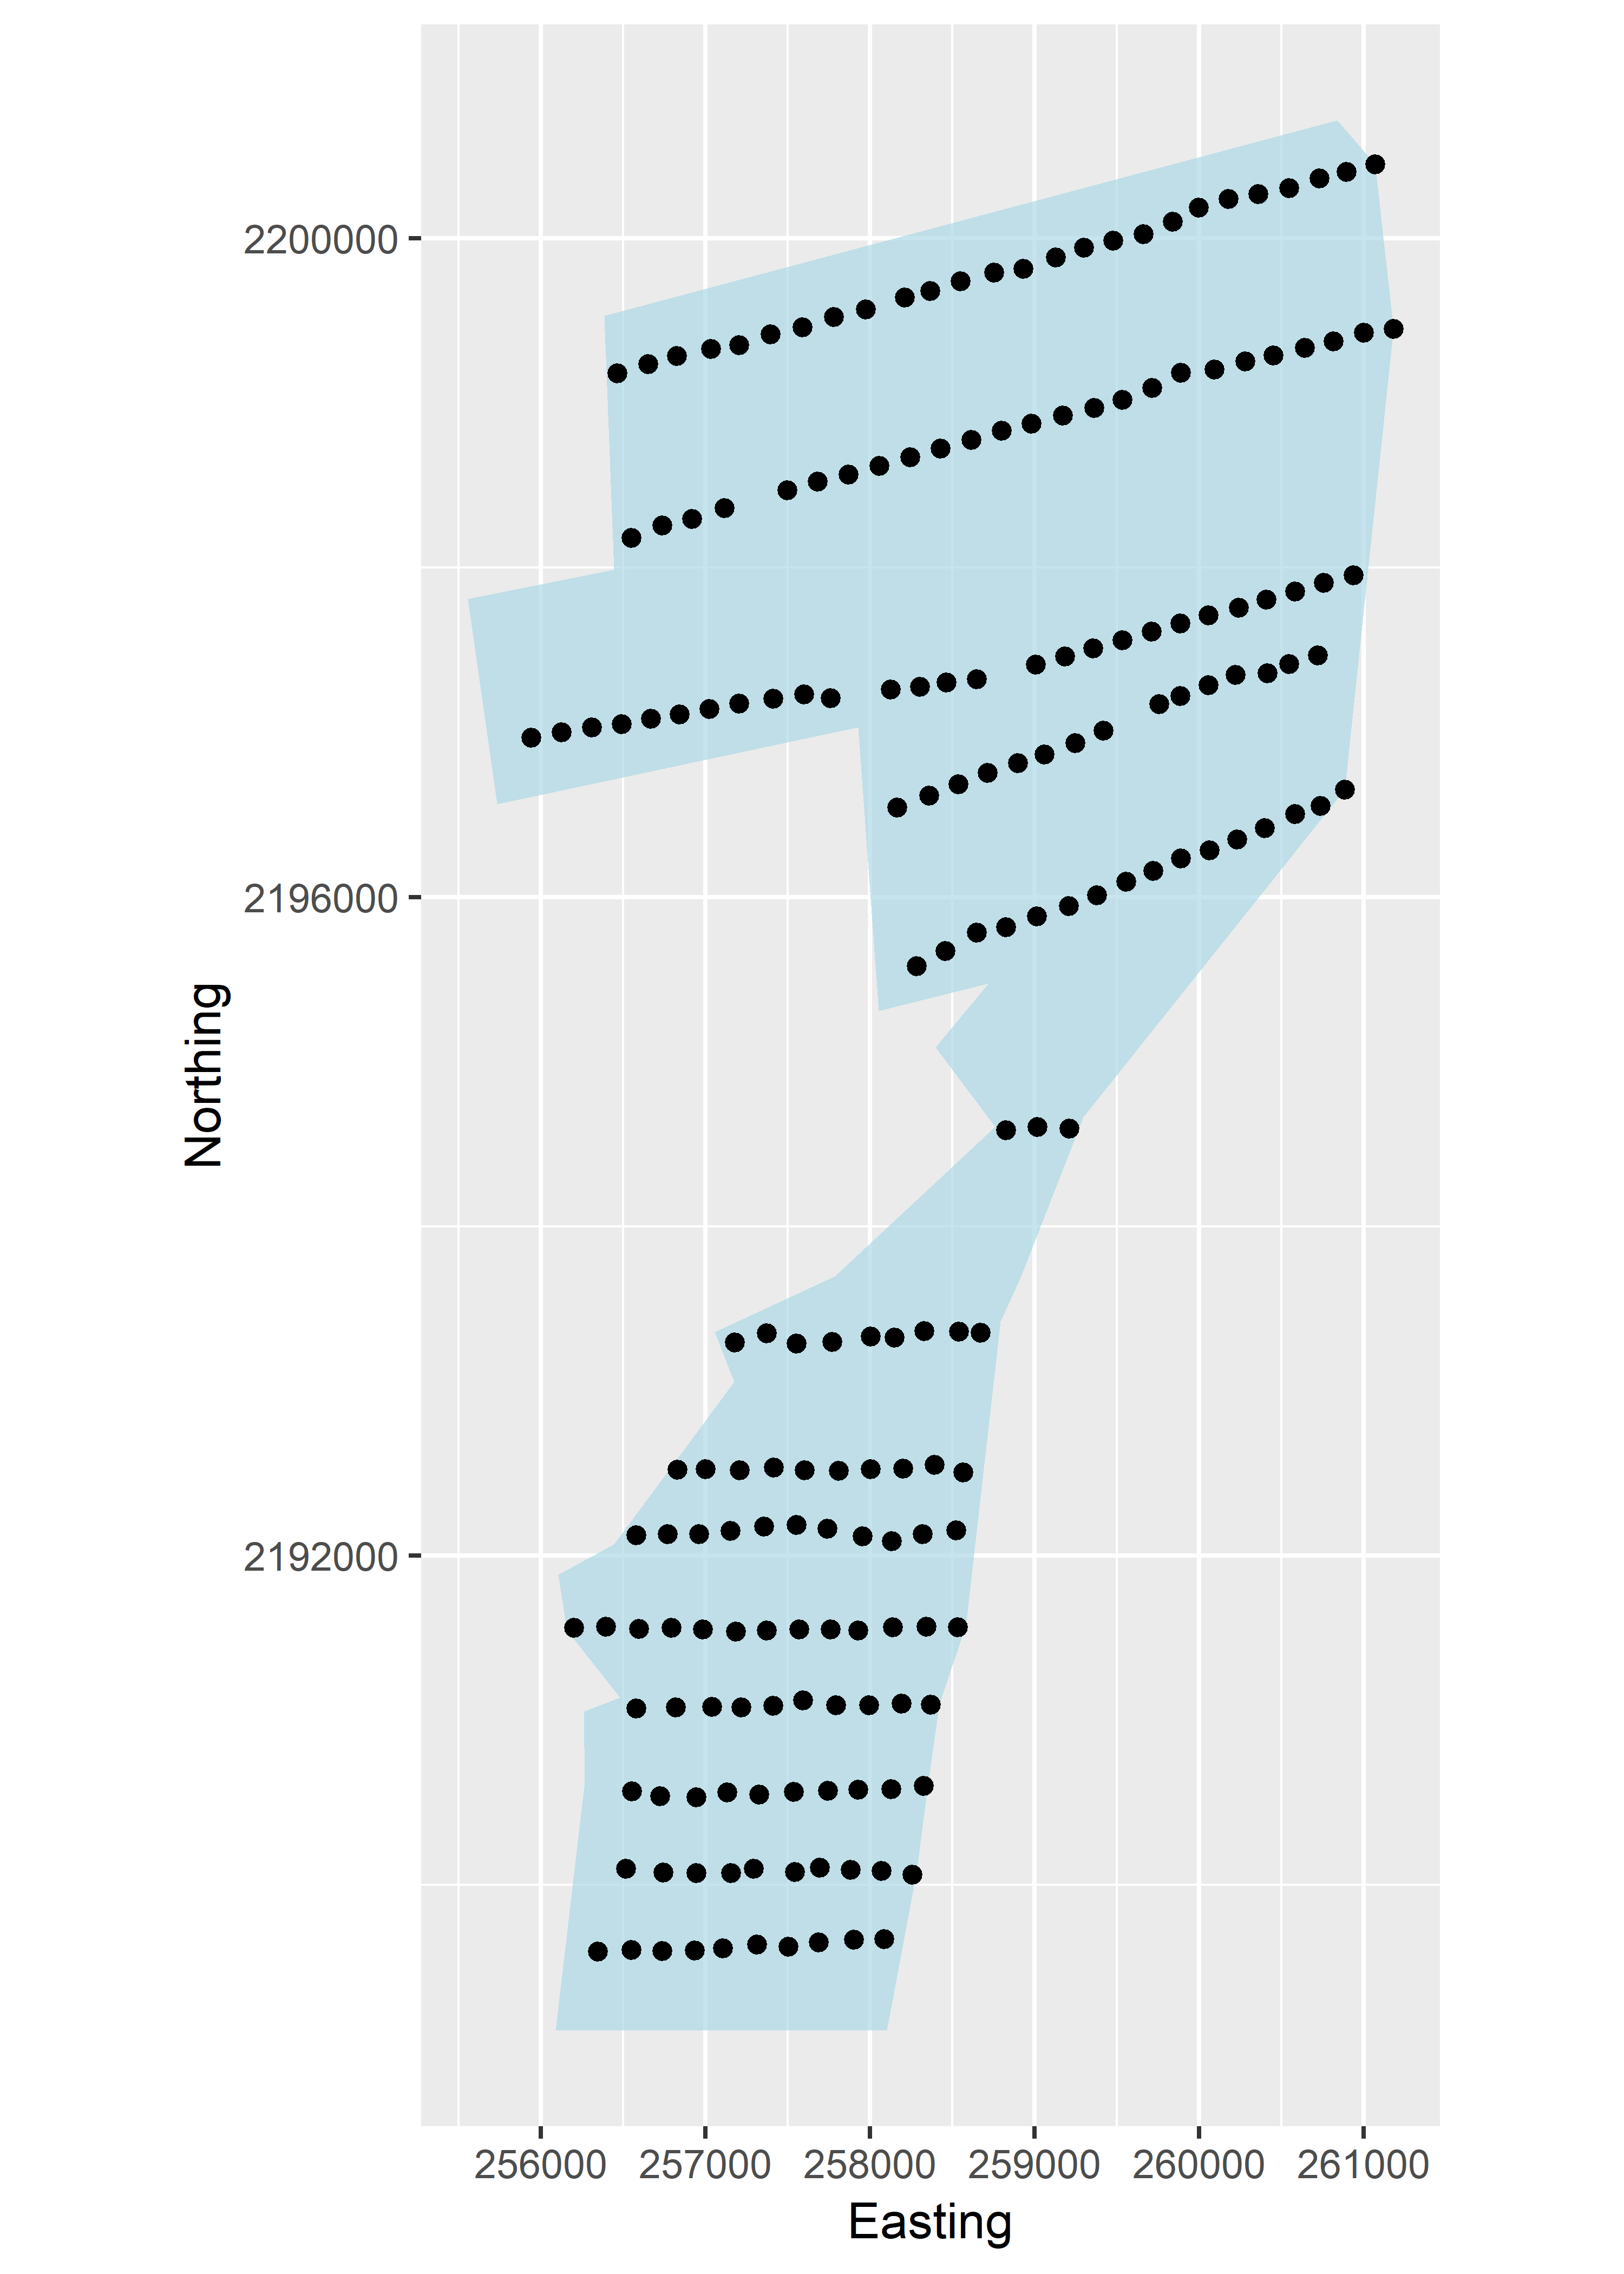
\includegraphics[scale=0.5]{figures/2002studyareapoints_pt}
	\caption{Study area (light blue) showing the 2002 survey points (black dots) in Hakalau Forest National Wildlife Refuge, \hawaii{} Island.}
	\label{fig:2002studyareapointspt}
\end{figure}

\subsection*{Bird sampling}
Surveys used point-transect methods, a form of distance sampling, where horizontal distances from survey points to individually detected birds are used to model a species-specific detection probability that is used to estimate absolute abundance and variance \citep{buckland_distance_2015}. Surveys commenced at dawn and continued until 11:00 or halted when weather conditions exceeded prescribed conditions that hindered detecting birds (light rain, and wind and gust strength \textgreater Baufort scale 3). During 8-min counts trained observers recorded the species, exact distance to the nearest meter and detection type for each bird detected, along with the sampling conditions cloud cover, rain, wind strength, gust strength, and time of day each point was surveyed.

\subsection*{Data description}
For purposes of our analysis, we selected a single survey from the \akepa{} time series based on broad sampling of the study area and sufficient numbers of detections. In 2002, 195 points were sampled using point-transect distance sampling methods within the 3,061 ha open-forest study area of Hakalau (Fig. \ref{fig:2002studyareapointspt}). On 67 points 152 \akepa{} were detected. The number of detections ranged from zero to 6 (Fig. \ref{fig:2002countspt}). These data are used for both the two-stage and one-stage model-based analyses. \cite{camp_population_2010,camp_statespace_2016} provide a detailed description of Hakalau, the open-forest study area and the bird surveys.

\begin{figure}
	\centering
	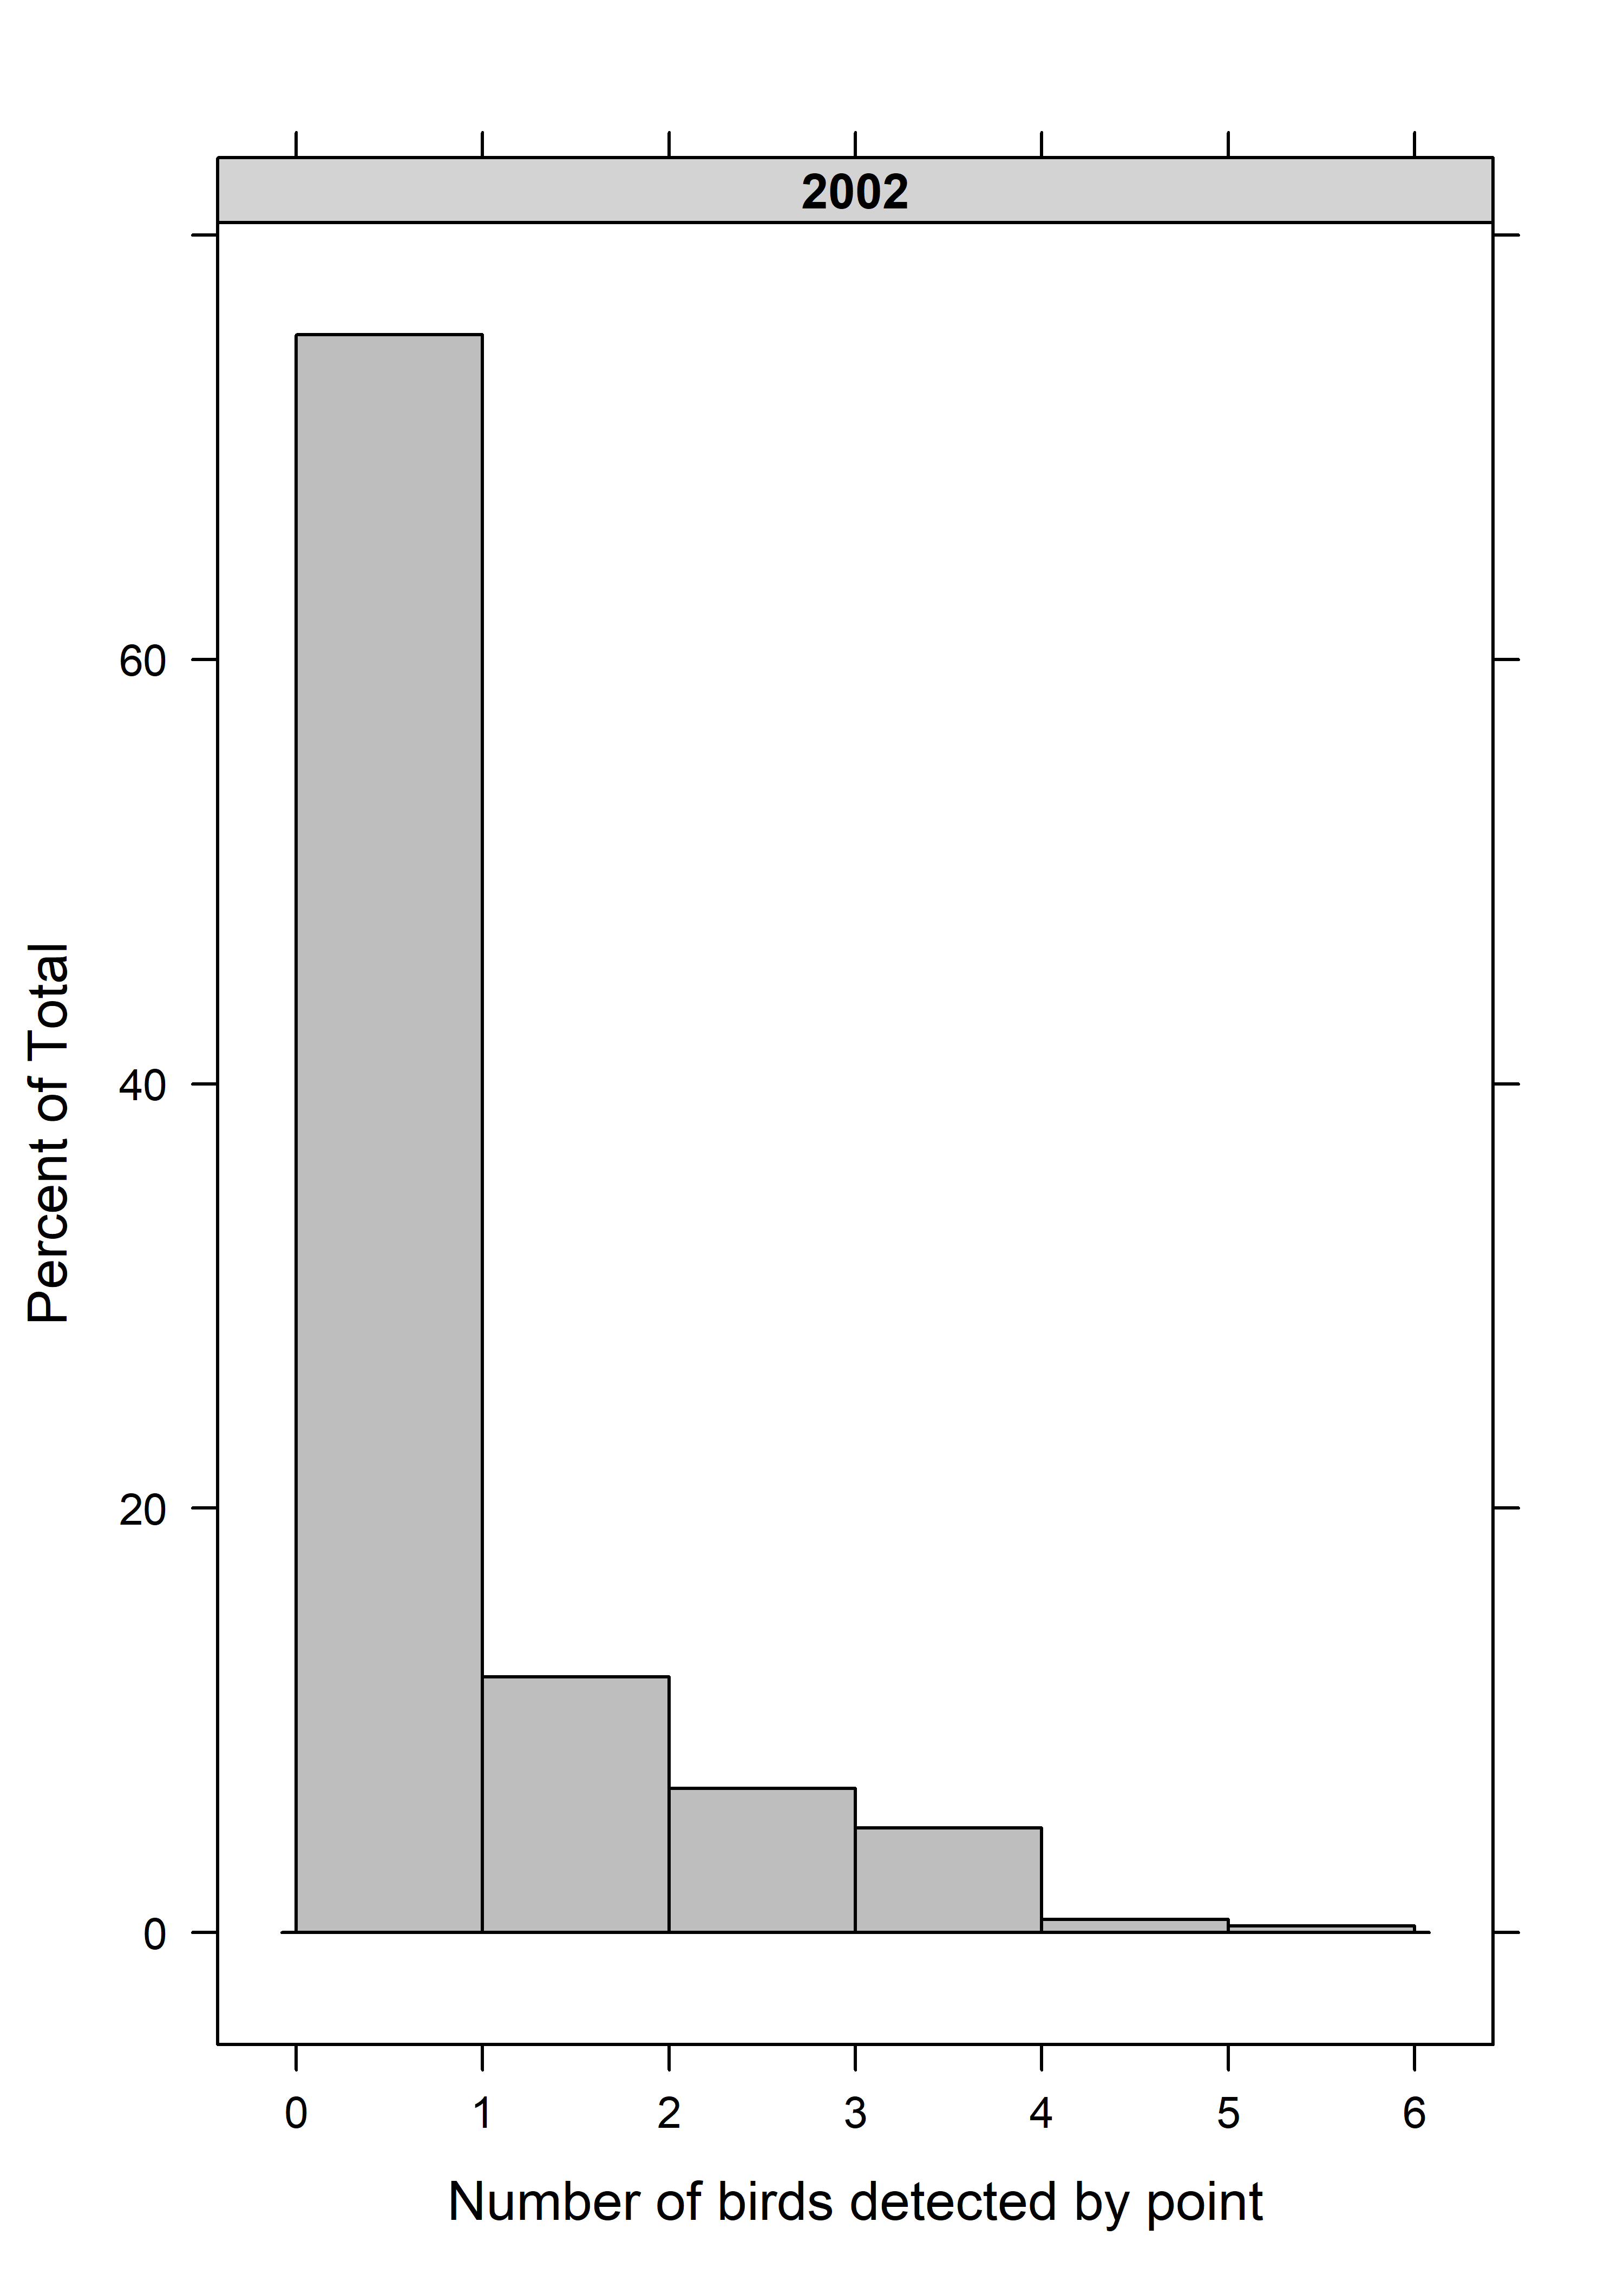
\includegraphics[scale=0.5]{figures/2002counts_pt}
	\caption{Counts of \akepa{} by point during the 2002 survey.}
	\label{fig:2002countspt}
\end{figure}

% addtextend

\subsection*{Model specification}

TODO HERE:  Add code snippets of how to specify the model in inlabru, brief discussion of PC priors and how they were chosen here

\subsection*{Results}

The predicted mean of the posterior intensity is shown in \autoref{fig:intensity-mean-cv} along with a map of the coefficient of variation (CV) of the posterior intensity field on a regular prediction grid with cell area of approximately 1.7 hectares.  This shows a region of high intensity in the south and much lower intensity in the north.  The CV plot shows clearly that there is less variation in the posterior intensity field in areas with greater sampling effort.  In general the south, with greater density of sampled locations, has a lower CV than the north, where sampling units are more spread out.  The areas of highest CV are those regions furthest away from any sampled location, reflecting the intuitive fact that we are least certain in areas further away from the sampled locations.  

\begin{figure}
	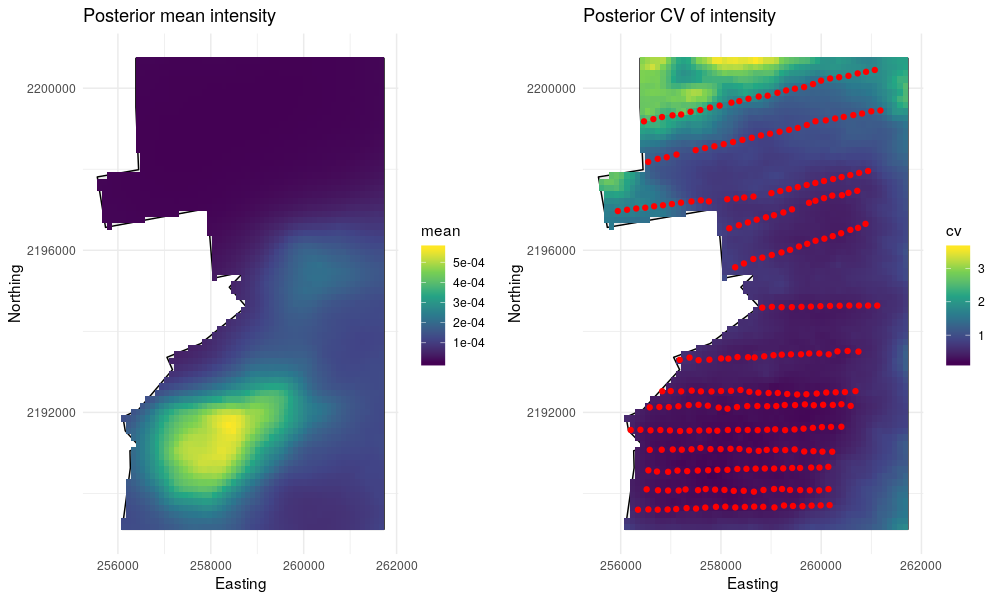
\includegraphics[scale=0.5]{figures/intensity_mean_cv.png}
	\caption{(left) Posterior mean of the intensity (right) Posterior coefficient of variation of the intensity}
	\label{fig:intensity-mean-cv}
\end{figure}

The CV plot shows a measure of uncertainty relative to the mean intensity in each prediction grid cell.  However, often we are interested in the uncertainty around the mean intensity on the scale of the intensity function itself - perhaps seeking to identify areas where we can confidently predict particularly high or low intensities.  To attempt to communicate this uncertainty around the mean it is common [[references?]] to present the lower and upper quantiles corresponding to a 95\% credible interval for each prediction cell (\autoref{fig:intensity-quantiles}). [RJC - I don't think a reference is needed to substantiate presenting credible intervals or computing them using quantiles, particularly in a stats journal. AES - I was trying to find an example of someone presenting maps like these in a paper, yet to find one.  If you know of any please let me know!]

\begin{figure}
	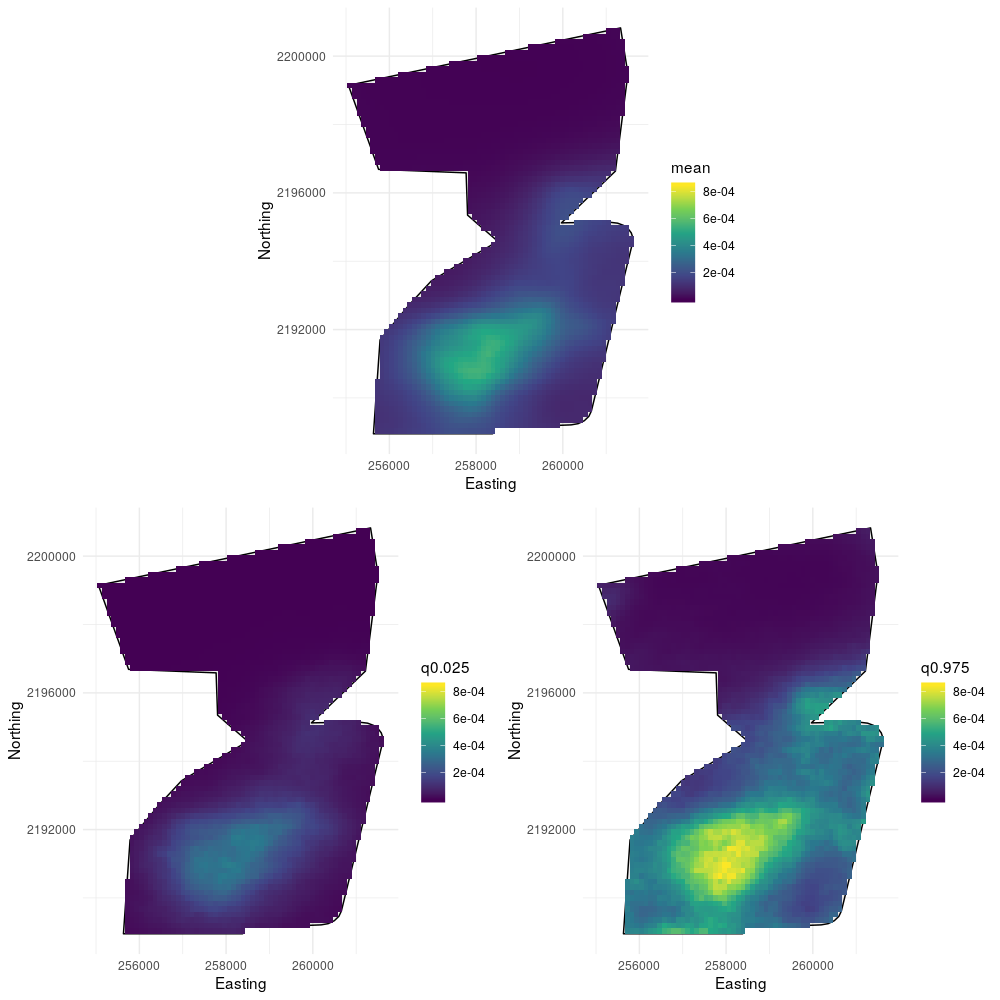
\includegraphics[scale=0.5]{figures/intensity_quantiles.png}
	\caption{The predicted posterior intensity summarised in three plots by the mean (upper),  0.025 quantile (lower left) and 0.975 quantile (lower right) for each prediction grid cell.  All three plots use a common colour scale}
	\label{fig:intensity-quantiles}
\end{figure}

We believe quantile plots like those in \autoref{fig:intensity-quantiles} to be challenging to interpret and potentially misleading.  The temptation is to interpet these plots as showing possible intensity surfaces that produced the observed data.  We believe this misconception would be extremely common in particular for non-statistically trained audiences. The maps in \autoref{fig:intensity-quantiles} in fact only show \textit{summary statistics} of a posterior intensity which is specified (in our model) as a log-Gaussian random field.

This difference becomes clear if one generates realizations of the posterior intensity field.  Three such realizations are in \autoref{fig:intensity-realizations}.  There are some notable differences when compared to the mean and quantile summary maps.  First, each realization has finer-grained spatial structure than the mean of the field.  In practice, this indicates that we should expect more spatial structure in our collected data than what we might expect if we only look at the posterior mean of the field.  The mean field plot hides the spatial structure the model has been able to estimate from the data.  In general, the mean of a random field will contain less spatial structure than realisations of the field. [RJC - 'First' is not followed up with subsequent ordinal numbers; I suggest rewriting the above sentence to remove 'first' or add ordinal numbers below.]

\begin{figure}
	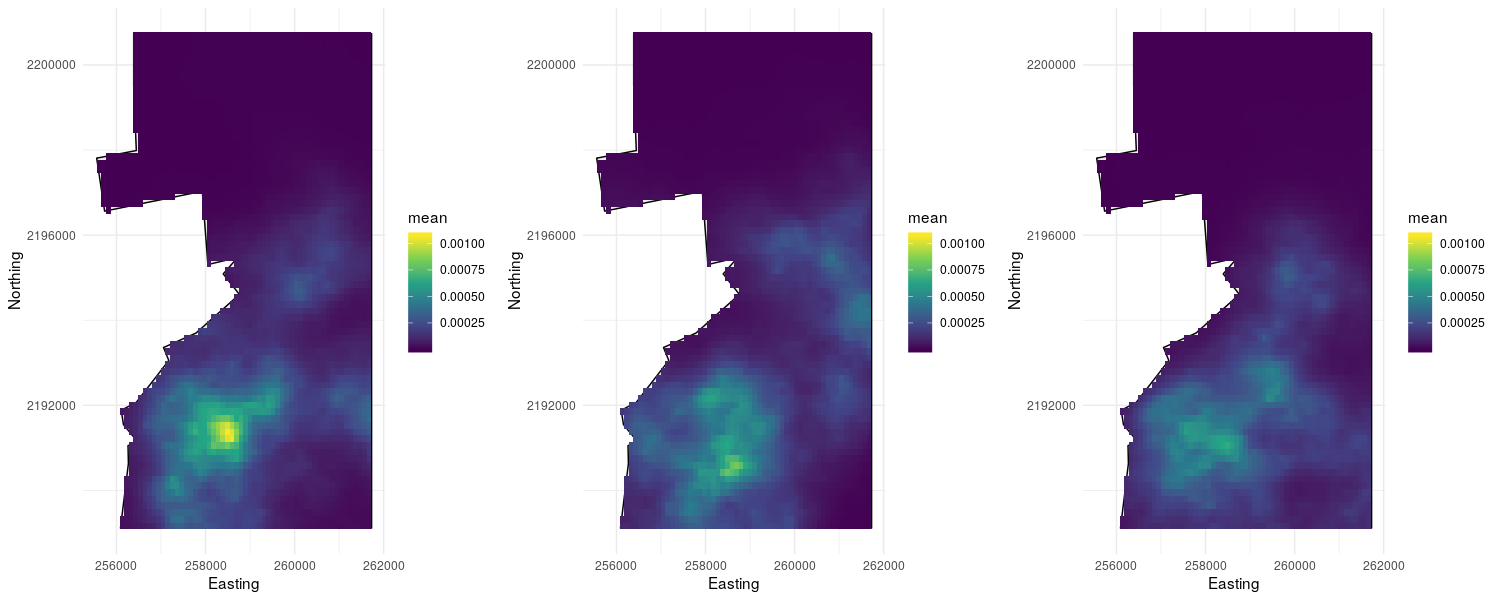
\includegraphics[scale=0.35]{figures/intensity_realized.png}
	\caption{Three realizations of the posterior intensity field}
	\label{fig:intensity-realizations}
\end{figure}

The quantile plots are more concerning.  As mentioned above, the temptation is to interpret these as possible intensities that produced our observed data.  However, they in fact show the quantiles of the \textit{marginal} probability density for each prediction location.  This essentially treats each prediction cell as independent of the others. Whilst any one prediction location may be well described by such quantiles, to present them side by side in one image obscures the fact that the probability that all (or some subset of) the prediction cells would \textit{simultaneously} achieve that value will be in fact much lower than the quantile value and in many cases would be essentially zero.  [RJC - I stumbled over this sentence several times and I think it needs to be rewritten.]  To demonstrate this we treated the lower and upper quantile plots as though they were intensities and integrated them to obtain an expected abundance estimate of approximately 2500 for the 0.025 quantile and 12,300 for the 0.975.  A naive (and tempting) interpretation of these numbers is as upper and lower limits of the 95\% credible interval for abundance. However, these abundance estimates are essentially impossible according to the estimated posterior for abundance (see \autoref{fig:realized-abundance-posterior}).  This emphasises that the temptation to treat these maps as showing possible intensity surfaces leads to outcomes (and possible management decisions) that are inconsistent with the very model that generated the maps.

As an alternative, we suggest using excursion sets and excursion functions \citep{bolin_excursion_2015}.  This is a recently developed approach to representing uncertainty in stochastic processes that specifically considers joint probability of events across multiple locations.  The positive excursion set with level $u$ for a function $f(s)$ with domain $\Omega$ is $A_u^{+}(f) = \{ s \in \Omega ; f(s) > u \}$ i.e. the set of all locations in $\Omega$ where $f$ exceeds the a threshold value $u$. For a stochastic process $\lambda(s)$ the positive excursion set with level $u$ and probability $1 - \alpha$ is

\begin{equation*}
E_{u,\alpha}^{+}(\lambda) = \argmax_{D}\{\lvert D \rvert : \mathbb{P}\left[D \subset A_u^{+}(\lambda)\right] \geq 1 - \alpha \}
\end{equation*}
It is important to note that $A_u^{+}(f)$ specifies a set for which a function $f(s)$ exceeds a threshold value $u$ for \textit{every location} in the set.  This means that when considering random quantities such as $\lambda(s)$ the definition of the positive excursion set $E_{u,\alpha}^{+}(\lambda)$ is the largest such set for which a threshold is exceeded simultaneously for all locations in the set.  Because $\lambda(s)$ is stochastic we can only ever say this is true with some probability and use something akin to a confidence level by specifying $\alpha$.

Excursion sets can be estimated by considering candidate sets for $D$ of increasing size and a sequential integration scheme to estimate probabilities.  An implementation is available in the \texttt{excursions} package \citep{bolin_calculating_2018} available through the Comprehensive R Archive Network \citep{r_2017}.

\autoref{fig:excursions} (left panel) shows the positive excursion set with a level corresponding to 1 bird per hectare with probability 0.95.  This figure can be interpreted in a natural way.  It is the largest possible region for which the intensity is greater than 1 bird per hectare for every location within the region, with probability 0.95.

\begin{figure}
	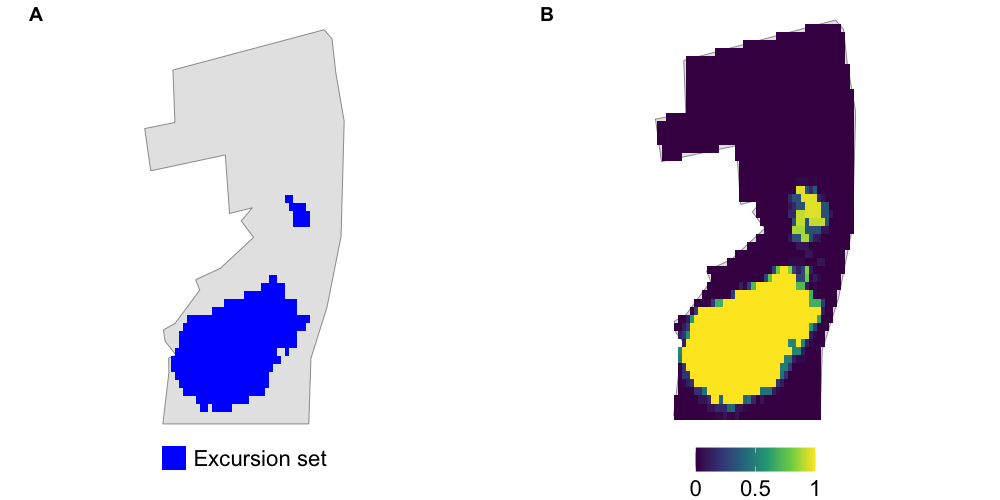
\includegraphics[scale=0.5]{figures/excursions.png}
	\caption{Left:  The positive excursion set with a level corresponding to 1 bird per hectare and probability 0.95.  Right: The positive excursion function with a level corresponding to 1 bird per hectare}
	\label{fig:excursions}
\end{figure}

To visualise multiple such maps we can use the excursion function $F_u^{+}(s) = \sup \{1 - \alpha ; s \in E_{u,\alpha}^+ \}$, which defines for each location something similar to a p-value.  For each $s$ it is the largest possible probability $1 -\alpha$ for which that location would be in the excursion set defined using probability $1 - \alpha$.  The excursion function with a level corresponding to 1 bird per hectare is shown in \autoref{fig:excursions} (right panel).

This figure can also be interpreted naturally.  It shows the largest possible probability for each location to be a member of a set for in which the intensity exceeds a threshold simultaneously across all locations in the set. Regions on the edge of the excursion set would be included if the $\alpha$ value were allowed to increase slightly.  However, for regions in the north there is essentially no probability level for which those locations would be included in $A_u^{+}(\lambda)$.

A key feature of these plots is that they display either discrete sub-regions of the area of interest (for excursion sets) or the probability of membership of such discrete sub-regions (for excursion functions).  We believe the risk of interpreting these maps as intensities is much lower than for the quantile plots.  The fact that it is possible to estimate discrete regions may also be useful to communicate results to conservation practitioners, land and resource managers and policy decision-makers.  We anticipate the excursion function will be most useful in communicating to audiences with statistical training. [RJC - I think statistically savvy audiences will readily grasp the excursion functions. Do you mean "without" statistical training?]

Another key aim of performing distance sampling surveys is to estimate the abundance of the population of interest.  By specifying our spatial model as a log-Gaussian Cox process, the posterior intensity is a random field rather than a deterministic function. Let $n$ denote the abundance of the population within the region of interest and $N$ its corresponding random variable within our Bayesian framework.  Integrating the mean of the random field provides a point estimate for the abundance, which we term the expected abundance.  Here we demonstrate the importance of considering the full posterior for $N$ which we call the \textit{realized} abundance.

Let $N = \int_{\Omega}\lambda(s)\mathrm{d}s$. Note that $N$ is a random variable and the integral of $\mathbb{E}[\lambda(s)]$ is equivalent to $\mathbb{E}(N)$ by Fubini's theorem, hence the term expected abundance.  As we mentioned above, this is the most sensible point estimate for the abundance.  We estimate the posterior $\pi(N | \lambda)$ by a monte-carlo method.  Taking $m$ monte-carlo samples  $\lambda_1, \ldots, \lambda_m$ of the posterior intensity field we estimate the posterior for the abundance as $\pi(N | \lambda) \approx 1 / m \sum_{i=1}^m \pi (N | \lambda = \lambda_i)$. This is well-defined since $\pi(N | \lambda = \lambda_i)$ is a Poisson probability mass function with rate parameter $\int_{\Omega}\lambda_i(s)\mathrm{d}s$. \autoref{fig:realized-abundance-posterior} shows the approximate posterior for $N$ with $m = 20,000$.  This allows us to estimate the probability for any specific value of \textit{realized} abundance $n$ by calculating $\pi(N = n | \lambda)$.  For reference, \autoref{fig:realized-abundance-comparison} shows a single Poisson PMF with rate parameter equal to the expected abundance.

\begin{figure}
	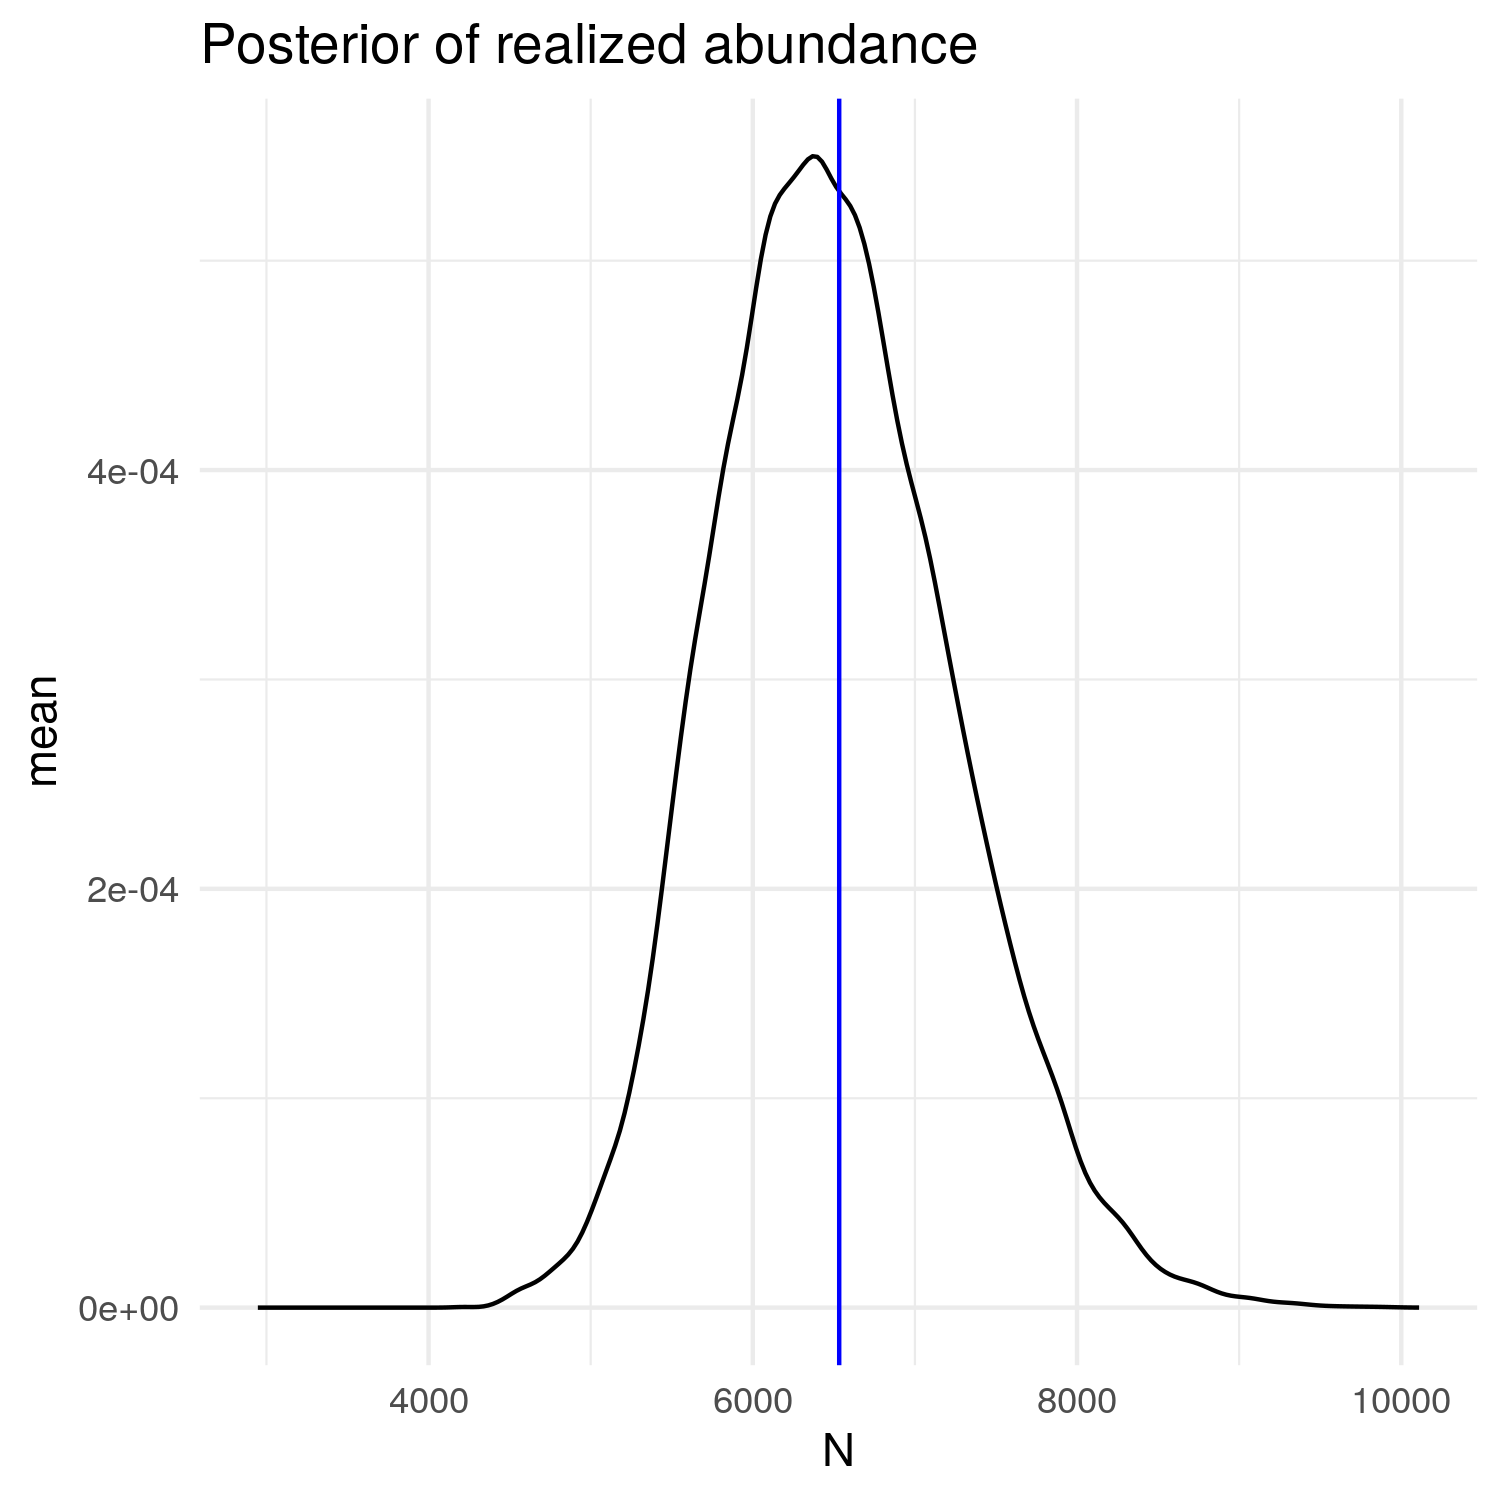
\includegraphics[scale=0.6]{figures/realized_abundance_posterior.png}
	\caption{Posterior of realized abundance.  The blue line marks the expected abundance}
	\label{fig:realized-abundance-posterior}
\end{figure}

\begin{figure}
	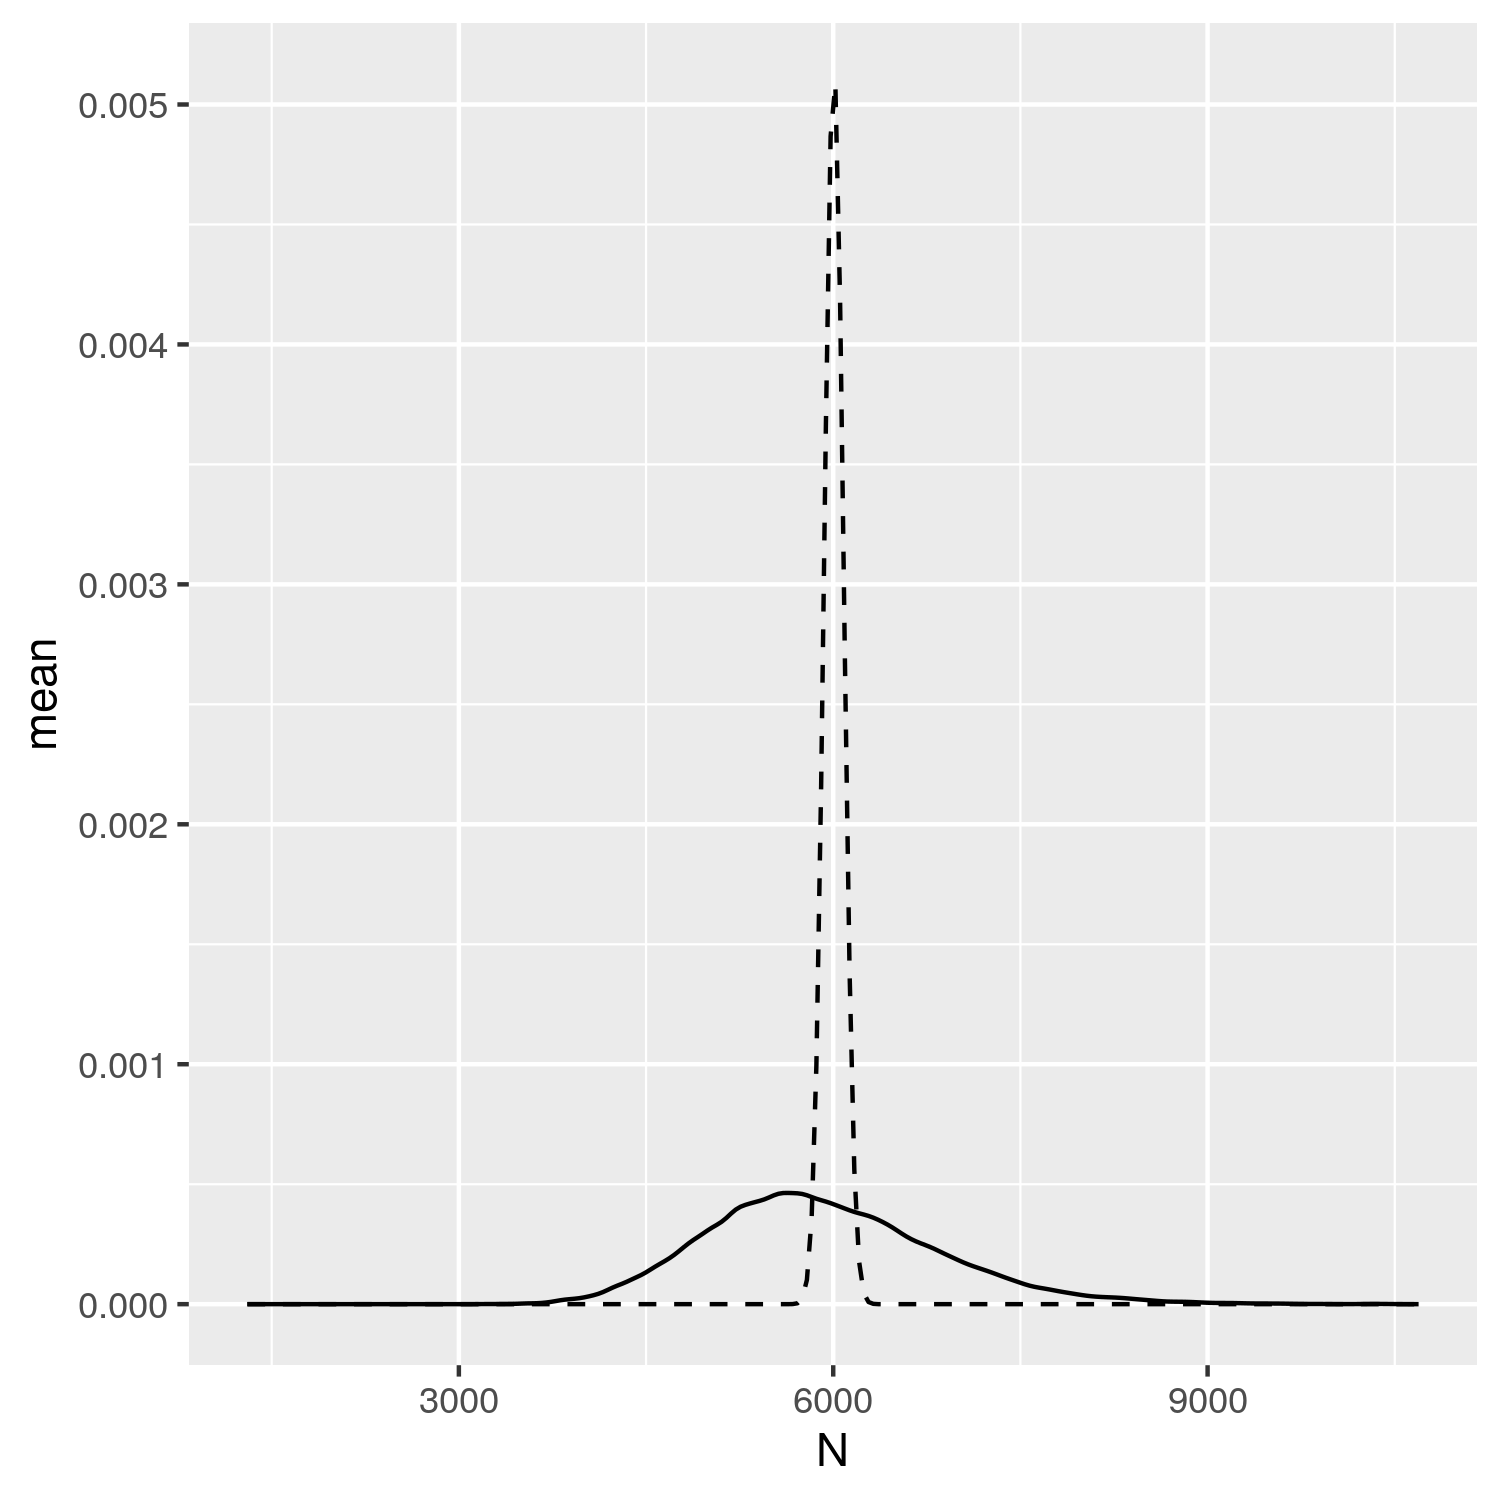
\includegraphics[scale=0.6]{figures/realized_abundance_vs_exp.png}
	\caption{Solid:  Posterior of realized abundance.  Dashed:  Poisson PMF with rate parameter $\mathbb{E}[\Lambda]$}
	\label{fig:realized-abundance-comparison}
\end{figure}


\begin{figure}
	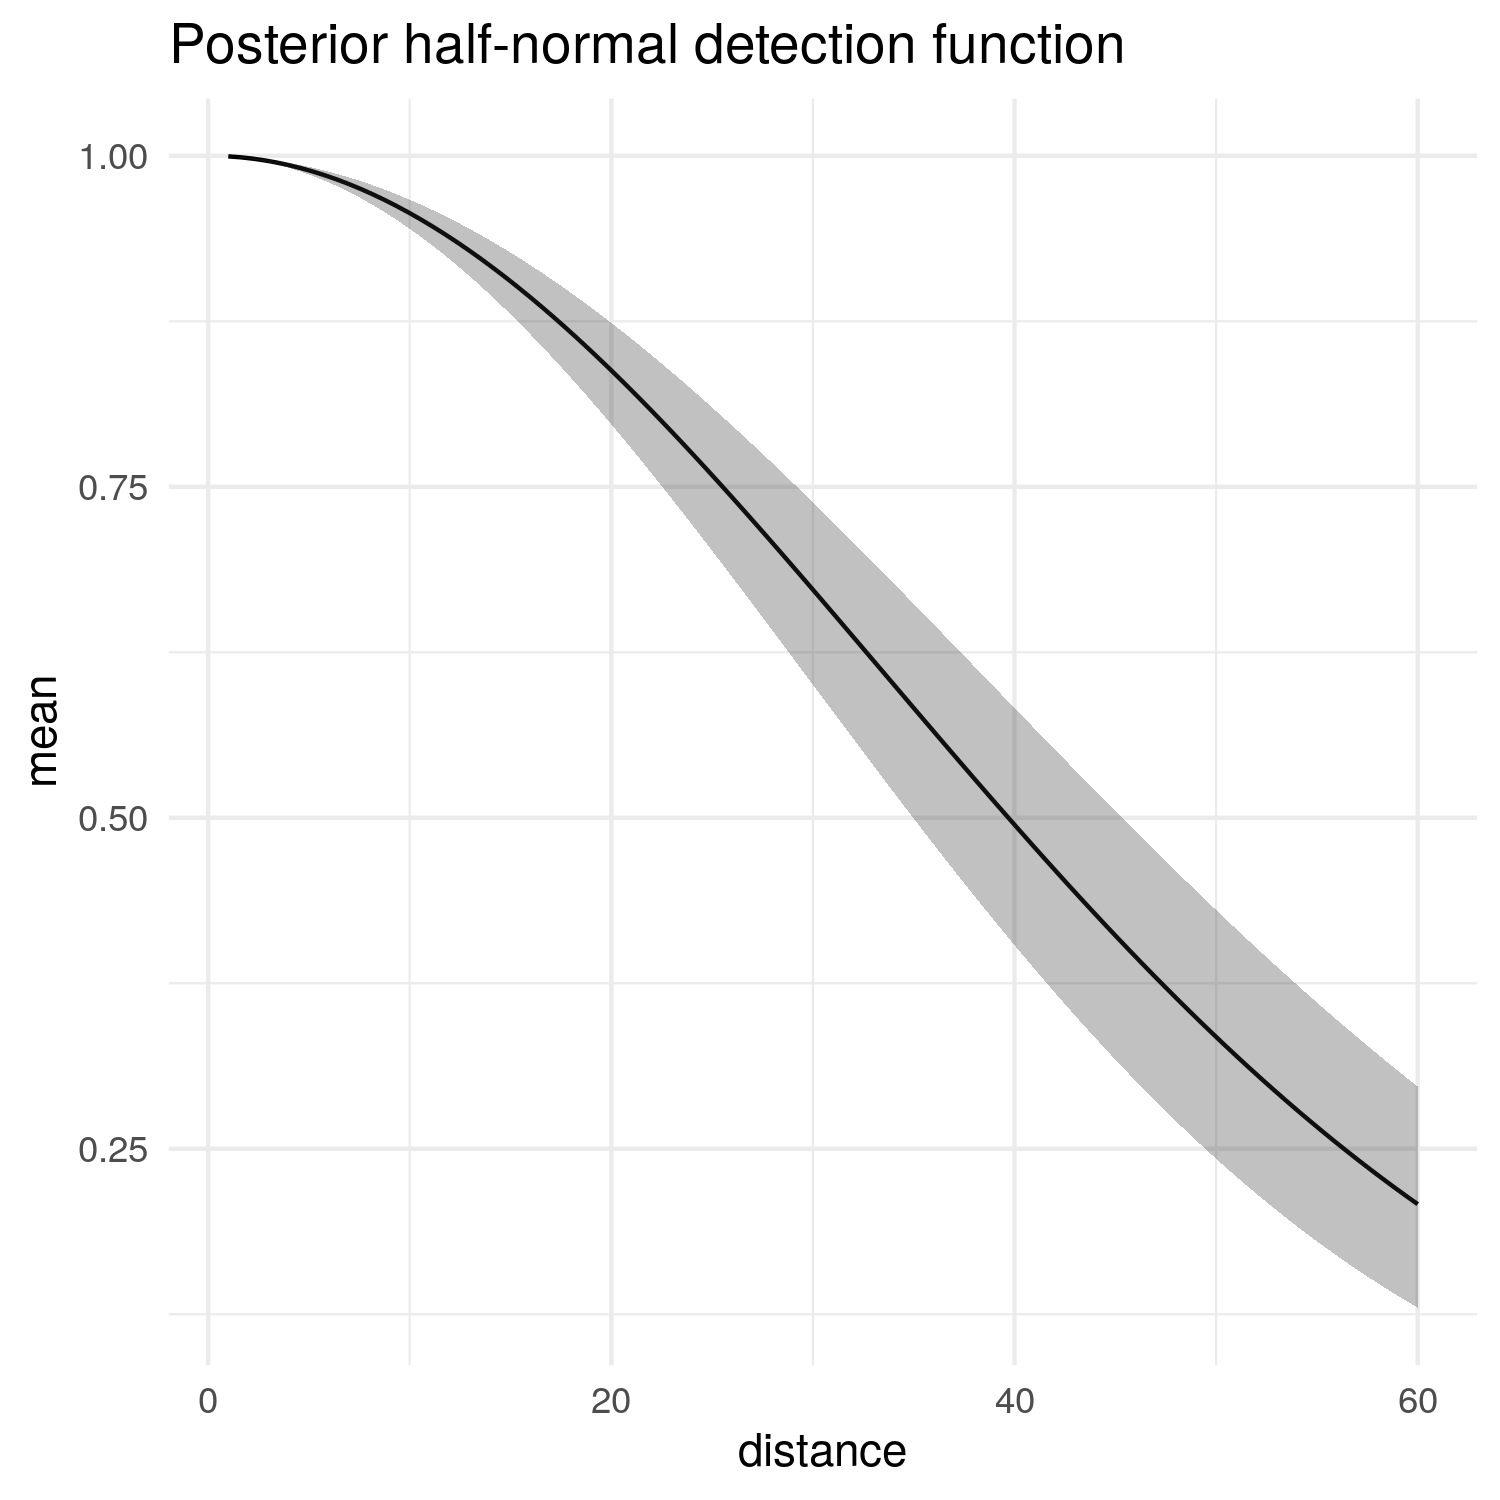
\includegraphics[scale=0.6]{figures/halfnormal.png}
\end{figure}

\bigskip

TODO HERE:  Something about how this is all a one-stage model and all these plots are based on sampling from the joint posterior of all parameters.  As such all plots can be viewed as incorporating the uncertainty from the detection model.  This is a lovely and natural way to present results and an advantage of having a joint model.  I'm not sure varprop can do this? [RJC - Varprop does do this through the posterior covariance $V_{\beta}$ matrix of the intercept, smoother and detection probability terms. But it doesn't do so in such an elegant way. Varprop is still reliant on a two-stage model.]

\newpage

\section*{Discussion}

\begin{enumerate}
	\item Note the model-based Bayesian hierarchical approach provides a framework for working with distance sampling data.  This allows simultaneous estimation of parameters associated with the detection process and the spatial distribution.  It is in principle extendible... somehow...

	\item Note that Bayesian distance sampling [RJC - References for this include Oedekoven et al (2014, JABES 19:219-239) and Buckland et al. (2015). We could also include Buckland et al. (2016, JABES 21:58-75) but it deals more with model-based design distance sampling than Bayesian approaches specifically. The more recent papers that reference Cornelia's paper are applied. It is also worth looking at Yuan's paper on point process models of blue whales.] has been done before but that the INLA approach avoids data augmentation and MCMC.
	\item Iterated INLA is a powerful and flexible way to include non-linear components to a predictor and has applications beyond this application to distance sampling
	\item More to do in future to test how many parameters can be included in the non-linear component and what types of non-linear components are feasible
	\item Note similarities and differences with two-stage GAM approach
	\item Note that presenting uncertainty in maps is difficult and excursion sets are a promising contribution relevant to many areas of spatial statistics.
	\item Links to species "range" estimates - excursions possibly useful here.
\end{enumerate}

\bibliographystyle{chicago}
\bibliography{paper}

\end{document}
